%%%%%%%%%%%%%%%%%%%%%%%%%%%%%%%%%%%%%%%%%%%%%%%%%%%%%%%%%%%%%%%%%%%%%%%%%%%%%%%%
%2345678901234567890123456789012345678901234567890123456789012345678901234567890
%        1         2         3         4         5         6         7         8

%\documentclass[letterpaper, 10 pt, conference]{ieeeconf}  % Comment this line out
                                                           % if you need a4paper
\documentclass[a4paper, 10pt, conference]{ieeeconf}        % Use this line for a4
                                                           % paper

%\IEEEoverridecommandlockouts                               % This command is only
                                                           % needed if you want to
                                                           % use the \thanks command
\overrideIEEEmargins
% See the \addtolength command later in the file to balance the column lengths
% on the last page of the document



% The following packages can be found on http:\\www.ctan.org
\usepackage{graphics} % for pdf, bitmapped graphics files
\usepackage{epsfig} % for postscript graphics files
%\usepackage{subfigure} % ben: is this package allowed?
%\usepackage{mathptmx} % assumes new font selection scheme installed
%\usepackage{times} % assumes new font selection scheme installed
%\usepackage{amsmath} % assumes amsmath package installed
%\usepackage{amssymb}  % assumes amsmath package installed

\title{\LARGE \bf
On Physics-Based 3D Waypoint Generation for Autonomous Exploration in Mobile Robotics
}

%\author{ \parbox{3 in}{\centering Huibert Kwakernaak*
%         \thanks{*Use the $\backslash$thanks command to put information here}\\
%         Faculty of Electrical Engineering, Mathematics and Computer Science\\
%         University of Twente\\
%         7500 AE Enschede, The Netherlands\\
%         {\tt\small h.kwakernaak@autsubmit.com}}
%         \hspace*{ 0.5 in}
%         \parbox{3 in}{ \centering Pradeep Misra**
%         \thanks{**The footnote marks may be inserted manually}\\
%        Department of Electrical Engineering \\
%         Wright State University\\
%         Dayton, OH 45435, USA\\
%         {\tt\small pmisra@cs.wright.edu}}
%}

\author{Benjamin Adler and Jianwei Zhang% <-this % stops a space
%\thanks{This work was not supported by any organization}% <-this % stops a space
%\thanks{H. Kwakernaak is with Faculty of Electrical Engineering, Mathematics and Computer Science,
%        University of Twente, 7500 AE Enschede, The Netherlands
%        {\tt\small h.kwakernaak@autsubmit.com}}%
%\thanks{P. Misra is with the Department of Electrical Engineering, Wright State University,
%        Dayton, OH 45435, USA
%        {\tt\small pmisra@cs.wright.edu}}%
}


\begin{document}



\maketitle
\thispagestyle{empty}
\pagestyle{empty}


%%%%%%%%%%%%%%%%%%%%%%%%%%%%%%%%%%%%%%%%%%%%%%%%%%%%%%%%%%%%%%%%%%%%%%%%%%%%%%%%

\begin{abstract}

This paper presents a novel, physics-based approach to computing waypoints and safe navigation, which are subsequently being used to steer a flying platform in three-dimensional space to map an outdoor environment. Because the algorithm relies on simple physical processes, it is both easy to understand and to implement in combination with traditional data structures. Generation of efficient sensor-trajectories for maximized information gain operates directly on unorganized point-clouds, creating a perfect fit for environment mapping with commonly user LIDAR sensors or time-of-flight cameras.

We also present the algorithm by simulating its performance in a virtual outdoor scenario.

\end{abstract}

%%%%%%%%%%%%%%%%%%%%%%%%%%%%%%%%%%%%%%%%%%%%%%%%%%%%%%%%%%%%%%%%%%%%%%%%%%%%%%%%


\section{Introduction}

Automatic model building has always been one of the most important parts of autonomous robotics. Exploration and mapping - as a subclass of this problem - has been the topic of many papers in recent years. The SLAM problem was first solved for two-dimensional mapping scenarios [nicht-thrun, freiburg etc.] and later-on expanded to three-dimensional environments [kinect-uav etc].

This paper presents a novel approach on increasing the efficiency of such mapping procedures. While the implementations of SLAM have improved greatly in recent years, one aspect of mapping three-dimensional environments was given comparatively little attention: finding the next best view. Typically, SLAM algorithms have been researched and developed on mobile platforms moving on flat surfaces[TODO]. This setup does not require a high efficiency in exploration, as it does not inherently impose time constraints. The authors of this paper, however, are implementing exploration and mapping algorithms on a flying platform with a maximum flight time of about 15 minutes. Aiming to explore as much of the environment as possible within this limited time motivates an efficient way of finding sensor-poses (and in extension, -trajectories) that enable sensors to deliver as much information as quickly as possible.

\section{State of the Art}

Since the introduction of Thrun's SLAM approach \cite{thrun_invented_slam}, much work has been done to refine and extend the algorithm for use in both two- and threedimensional environments [...]. Finding the next best view, though, has never been a part of the SLAM problem and is thus rarely addressed by these works.

Generating safely reachable waypoints from previously acquired sensor data is an extension of next-best-view problem, as it does not include the constraints of safe navigation. In general, frontier-based approaches are a popular method to compute new waypoints [1,2,3,4] as sensor-poses from areas between known and unknown environment offer a good compromise between safe reachability and high information gain. Unfortunately, information about frontiers between known and unknown space is hard to generate from three-dimensional datastructures such as pointclouds or octrees.

\subsection{Data structures}

Occupancy grid maps - and in extension elevation maps - are often used to store sensor data in generalized form. Although the data structure permits easy traversability computation and frontier detection, storing more complex geometry or overhangs remains difficult or even impossible, limiting its practical use to two-dimensional environments. Furthermore, its uniform grid size requires a global compromise between model quality and memory consumption. Multi-Level surface maps, introduced by Triebel et al [triebel], eliminate many of these limitations, while still being constrained to a grid.

In order to capture sensor data representing arbitrarily complex geometry and detail, we decided to implement our algorithm on an octree-based data-structure. Octrees are well suited for storing information in non-uniform resolution and the process of storing and retrieving data can easily be executed in parallel, allowing for optimization of parts of our algorithms. Besides its position, each point in the octree also stores its brightness (i.e. intensity as measured by the laserscanner) and a vector pointing from that point back to the sensor. As the platform's measured orientation is less precise that its measured position, this information will be used lateron to assign points recorded from further distance (and thus suffering a greater impact from platform-orientation errors) a lesser weight in the following surface reconstruction.

\section{Our approach}

\subsection{Platform}

\begin{figure}[thpb]
  \centering
  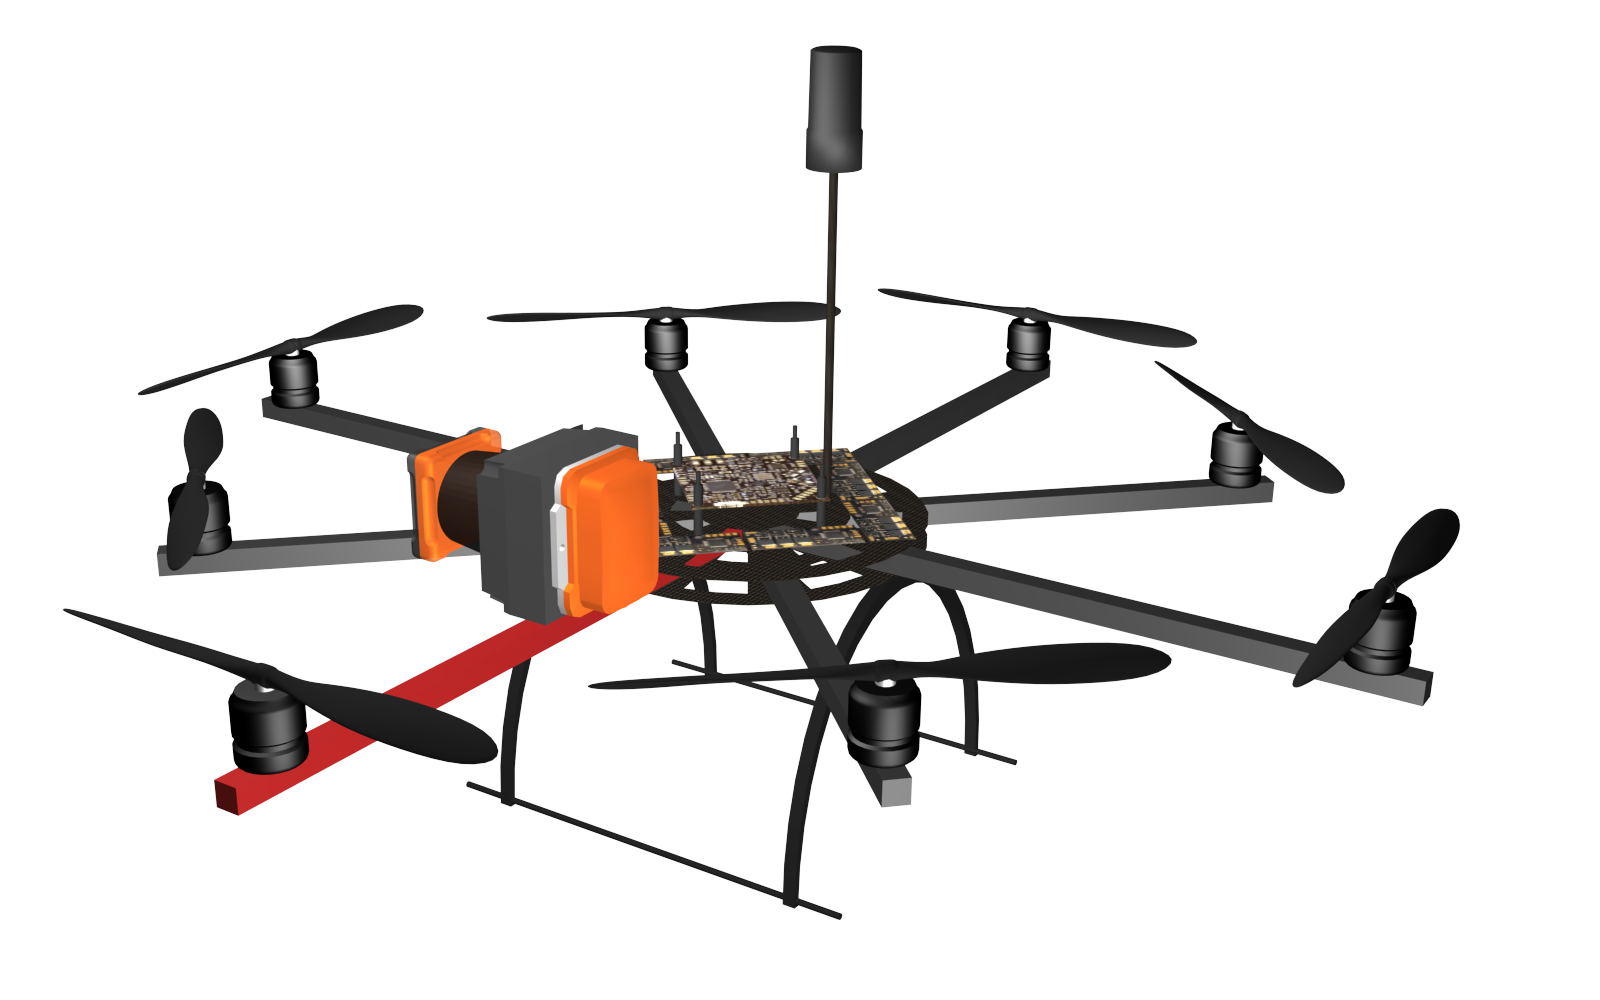
\includegraphics[width=0.5\textwidth]{images/oktokopter}
  \caption{Rendering of our experimental flying platform}
  \label{oktorendering}
\end{figure}

To save time during the construction of our platform, we used an ``Okto 2''-octocopter from the mikrokopter-project \cite{mikrokopterproject} as a base for our vehicle. Its central FlightControl (FC) processor-board is connected to eight brushless-motor controllers (BL) via an I2C bus. Employing its on-board gyros and accelerometers, the FC is programmed to stabilize the platform by itself when no other motion-control-commands are received from either the connected remote-control-receiver or via the serial port. The project also developed the NaviControl (NC), an add-on hardware module that sends motion-control-commands (thrust, yaw, pitch and roll each as 8-bit signed integers) to steer the platform to waypoints. We abandoned the idea of using the NC for our purposes, as its hardware lacks some flexibility, adds extra weight and its control-algorithms are not open-source.

Instead, we fitted an Intel Atom processor-board to the base. This board has a serial connection to the FC, which is used to send motion-control-commands and receive sensor input. Furthermore, we mounted a Hokuyo UTM-30LX laserscanner to the platform's front arm such that its scanning-plane is perpendicular to the platform's groundplane (as seen in Fig. \ref{oktorendering}).

A Septentrio AsterX2i RTK-GPS receiver has been installed and connected to an XSens MTi IMU, enabling measurement of the platform's pose at 20Hz. Due to RTK-GPS, the position is accurate to within 5cm while the orientation shows a maximum error of ~1� for pitch and roll and ~3� for yaw angles. To shield the GNSS-receiver from electrostatic interferences caused by the processor board and protect from physical damage, both have been encapsulated into electrically shielded carbon-fiber boxes.

The laserscanner rotates at 2400rpm and provides both falling and rising edges after each single scan. This signal is connected to the GPS-receiver, which is configured to emit the GNSS-time of the event with microsecond-precision on its USB-connection to the Atom processor-board. With both poses and laserscanner-events being timestamped by the GNSS-receiver, interpolation of the vehicle's pose to the scanner's pose at the time of each scan becomes possible.

% TODO: figure 1: two laserscanners. figure2: one laserscanner
We initially planned to use one laserscanner with its scan-plane perpendicular to both the platform's groundplane and its forward-vector for scanning the environment and another scanner oriented to have its scan-plane parallel to the vehicle's ground-plane for collision-avoidance (see Fig. \ref{lidar-setup-pair}). Besides the obvious disadvantages of another 250 grams of payload and ~10W of power consumption, the platform would have had to constantly pitch during flight to ensure reliable obstacle scanning and detection. To avoid these drawbacks, we instead mounted a single laserscanner as depicted in Fig. \ref{lidar-setup-single}. By constantly yawing the platform in flight, our single scanner captures both geometry for surface reconstruction and collision avoidance, provided that the platform does not move further than the laserscanners range within one rotation.
% TODO: speed < lidar-range * drehgeschwindigkeit ?

After balancing the platform's extra loads, it exhibits very favorable flight dynamics and drifts very slowly when idling. A switch on the remote control can be used to toggle between remote-control and computer-control. In the latter mode, the engines thrust will never exceed the value set on the remote control, providing ideal conditions for testing motion controllers. Including payload and battery, the platform weighs 2250 grams and requires around 350W of power while hovering, leading to a flight-time between 10 and 15 minutes.

\subsection{Algorithm}

\begin{figure*}[ht]
  \centering
    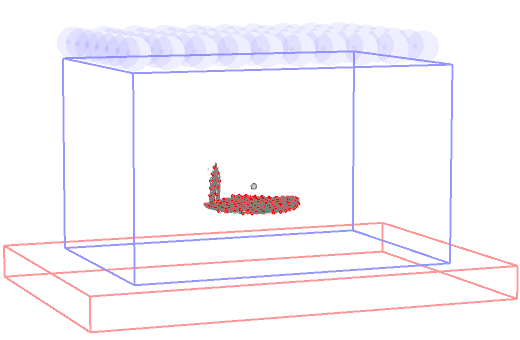
\includegraphics[width=0.23\textwidth]{images/expl1}
    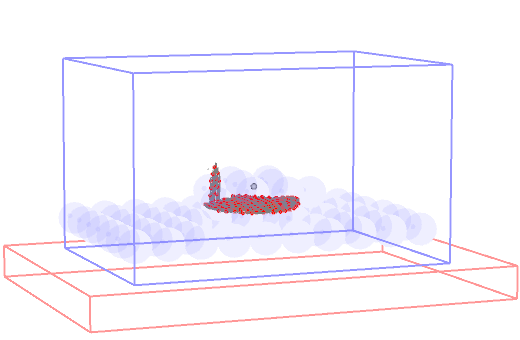
\includegraphics[width=0.23\textwidth]{images/expl2}
    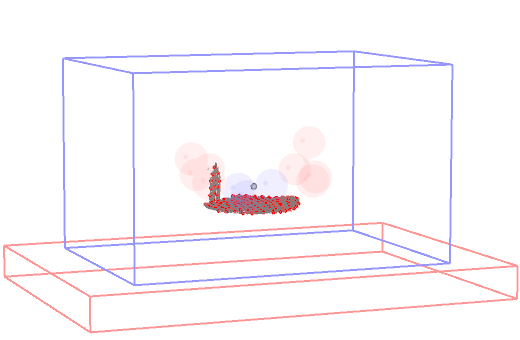
\includegraphics[width=0.23\textwidth]{images/expl3}
    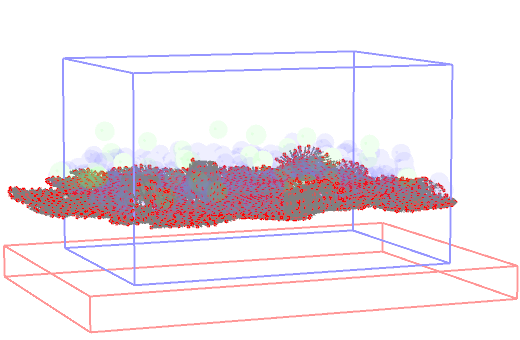
\includegraphics[width=0.23\textwidth]{images/process5}
    \caption{Mapping setup; bounding volume is blue, detection volume is red, vehicle position is grey, pointcloud for geometry reconstruction is grey and pointcloud for waypoint generation is red. Second figure shows sampling geometry interacting with pointcloud. Geometry hitting the red volume will be converted to a waypoint at the position it last hit a point from the pointcloud. The last figure shows generated pointcloud and leftover sampling geometry.}
    \label{explanation_of_process}
\end{figure*}

As three-dimensional environment mapping is often implemented using laserscanners and time-of-flight cameras, unorganized point clouds are a very common type of sensor data. Any sensor generating spatial occupancy information can be used, as the pointcloud is the algorithm's only input. Finding the next best view in such data be very hard, as the data itself does not supply any information about geometric structures such as corners, edges, surfaces and normals. Instead of trying to generate these details from the point cloud whenever it changes, our algorithm does not require such information.

While scanning, the pointcloud itself is saved into two customized octrees which differ only in the maximum density of points. One octree is used to capture all geometry for later surface reconstruction and thus allows for a very high density of points. The other octree is used for collision detection and stores points only if there are no other points whithin a distance of *dMin*, leading to comparatively little memory consumption. This density limitation is implemented by simple neighbor-queries common in most octree implementations. The exact purpose of this second octree will be explained soon.

Prior to the mapping process, the user creates a bounding volume as a representation of the region-of-interest around the vehicle's starting position, thereby defining the environment that is to be mapped. All generated viewpoints will be constrained to this volume, ensuring that the UAV does not leave the given area. At initialization, a physics engine is set up with a detection volume below the defined bounding volume. The contents of the collision-octree are automatically registered as collision objects int he physics world. After the octrees are populated with an initial set of points, the waypoint-generation algorithm is executed as follows:

\begin{enumerate}
     \item Create and initialize sample geometry: spheres of arbitrary size are created along the bounding volume's top plane.
     \item Start the physics simulation, allowing the sample geometry to follow the defined gravity. Whenever a sample sphere collides with a point registered in the collision octree, that event is saved into a special data structure mapping every sphere to the position of its last collision.
     \item When a sample geometry collides with the detection volume, it is removed from the simulation and the position of its last collision is recorded as a waypoint.
\end{enumerate}

Although any geometry can be used for waypoint generation, using spheres yields three important advantages:
\begin{itemize}
  \item Spheres can represented only by radius and position, so the overall memory requirement is very low (especially when all spheres share a common radius).
  \item Collision detection between points and spheres is a process of low computational complexity, even redundantizing the midphase in collision detection. To detect a collision, it is sufficient to check whether the distance between the sphere's center and the point is smaller than the sphere's radius.
  \item Most importantly, spheres are ideally suited to slip through smaller ``holes'' in the pointcloud, enabling their detection.
\end{itemize}

%Spatially limited by defined exploration space, other input pre-existing sensor information and vehicle position.

%Simulated annealing.


\subsection{Information Gain}

\begin{figure*}[ht]
  \centering
    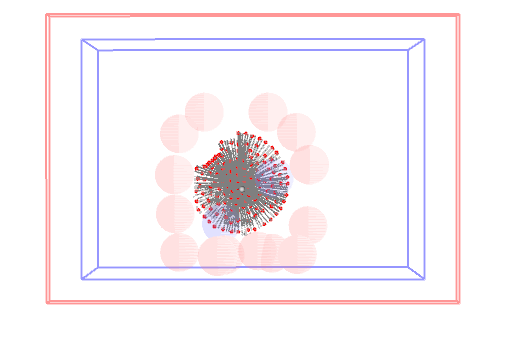
\includegraphics[width=0.2\textwidth]{images/process1}
    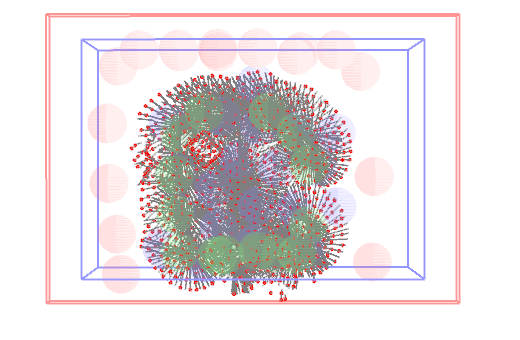
\includegraphics[width=0.2\textwidth]{images/process2}
    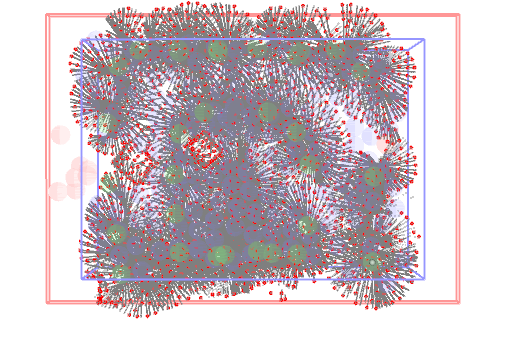
\includegraphics[width=0.2\textwidth]{images/process3}
    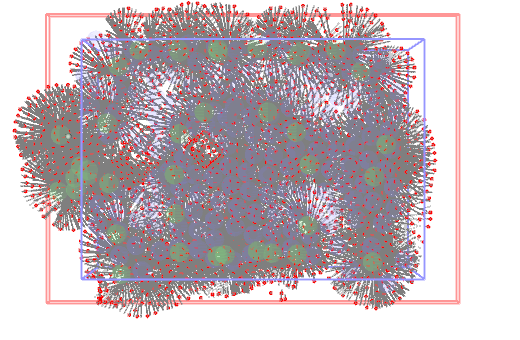
\includegraphics[width=0.2\textwidth]{images/process4}
    %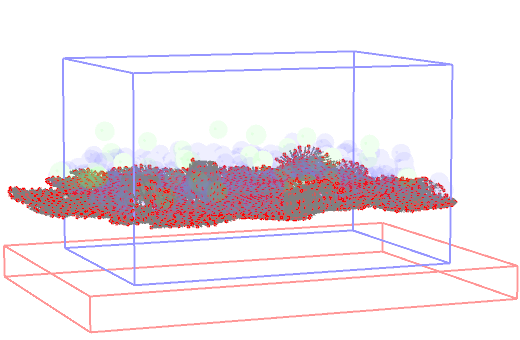
\includegraphics[width=0.2\textwidth]{images/process5}
    \caption{Multiple iterations of waypoint generation lead to a continuous scanning at the border between known and unknown environment.}
    %\label{expl3}
\end{figure*}

weil die kugeln, die von der kante fallen, (am meisten) z�hlen, bekomme ich immer wegpunkte mit dem gr��ten information gain?!

\subsection{Computational complexity}

The algorithms complexity derives from the computational effort of the collision detection phase in physics simulation and thus from the number of collision objects. Collision detection between $n$ objects in general requires $n(n-1)/2$ collision checks to be performed, leading to a complexity of O($n^2$). Optimized algorithms like sort-and-sweep or implementations relying on spatial subdivison may reduce the complexity to O($n$ log $n$) in favorable cases \cite{legrand2007}. This initially appears to be a major obstacle to employment of the algorithm outside of simulation, as the pointcloud may grow to several million points during a scan. Fortunately, the following optimizations have made the algorithm sufficiently fast for real-time application:

\begin{itemize}
  \item Given a pointcloud consisting of $n$ points and a set of $m$ sample geometries, the algorithm does not require collision tests between all $n+m$ objects. As the $n$ points making up the accumulated scan data are static, the number of required tests is reduced to $\frac{m(m-1)}{2} + n*m$. Because $n >> m$, this optimization yields a considerable loss in computational effort.
  \item When using the sensordata solely for waypoint generation, the density of the pointcloud can be reduced to allow gaps almost the size of the sample geometry's radius. That is, if sample spheres are created with a radius of e.g. 1m, the interacting pointcloud may discard points if there are neighbors within a distance of less than ~2m. In practice, this means a reduction of $n$ by two or three dimensions. For this reason, we use two pointclouds in our work; one is used for surface reconstruction and is stored in an octree which allows for close neihgbors (and thus high density) and another pointcloud used for waypoint generation and collision avoidance, stored in an octree rejecting points that would increase local density above the needed threshold.

  % The introduction of a second octree for collision detection is, in theory, unnecessary, as all of the pointcloud could be registered as collision objects in the physics world. In practice, however, using a second octree with a much lower point density dramatically reduces the number of collision pairs that have to be checked in every step of the physics simulation. This reduction translates to an increased efficiency, making the approach feasible for real-time application on current-generation CPUs.

  \item As described in Le Grand's work \cite{legrand2007}, execution of the simulation's broadphase on GPU can speed up execution by an order of magnitude compared to calculation on the CPU.
\end{itemize}

scalable resolution (sample sphere size / octree density)
simulated annealing length

\section{Experiments}
efficiency / performance
graph zeit vs number of points scanned
scalability durch Kugelgr��e / Menge

\section{Outlook}

With the algorithm relying on collision detection between many static and dynamic objects, it is currently limited by the speed of collision detection. Physics-simulation in general and collision detection especially tends to lend itself well to parallelization using massively-parallel implementations on GPUs

more efficient with opencl -> from iterative to realtime
kugeln spucken in flugrichtung

collision avoidance! lass die kugeln liegen, fliege dr�ber, dann wird nichts passieren?!

%\section{ACKNOWLEDGMENTS}
%The authors gratefully acknowledge the contribution of TAMS.

\begin{thebibliography}{99}

% ``Autonomous Exploration for 3D Map Learning'' by Johoo et al.



\bibitem{legrand2007}
% macht broadphase per CUDA, gut erkl�rt in GPU gems 3, chapter 32
Scott Le Grand, Broad-Phase Collision Detection with CUDA, {\it GPU Gems 3, } (2007)

\bibitem{gonzalez-banos2002}
% SLAM does not address the sensor-placement
% Extension to the ArtGallery-Problem
% Sensorkeulen von Kandidatenpunkten berechnen, 2D only
H\'{e}ctor H. Gonz\'{a}lez-Ba\~{n}os and Jean-Claude Latombe, Navigation Strategies for Exploring Indoor Environments, {\it I. J. Robotic Res.} 21(10-11), 829-848 (2002)

\bibitem{haehnel2004}
% Pioneer und Sick zu Outdoor Modellen, 16seiten, kein Wort �ber next-best-view
Dirk H\"ahnel and Wolfram Burgard and Sebastian Thrun, Learning Compact 3d Models of Indoor and Outdoor Environments with a Mobile Robot, {\it Elsevier Science Special Issue Eurobot} '01, 1-16

\bibitem{strand}
% Next-best-view centered
% Grid, 2d only
Marcus Strand and R�diger Dillmann, Grid based next best view planning for an autonomous robot in indoor environments

\bibitem{mikrokopterproject}
Mikrokopter project, http://www.mikrokopter.de, 2011

\bibitem{strand2008}
Marcus Strand and R�diger Dillmann, Using an attributed 2D-grid for next-best-view planning on 3D environment data for an autonomous robot

\bibitem{c2}
H. Kwakernaak and R. Sivan, {\it Modern Signals and Systems}, Prentice Hall, Englewood Cliffs, NJ; 1991.

\bibitem{c3}
D. Boley and R. Maier, "A Parallel QR Algorithm for the Non-Symmetric Eigenvalue Algorithm", {\it in Third SIAM Conference on Applied Linear Algebra}, Madison, WI, 1988, pp. A20.

\end{thebibliography}

\end{document}

